% !TEX root =  ../main.tex
\section{Preserve}

\subsection{Definition} 

\subsubsection{Signature} \cstr{preserve(s : set<VM>, r:string, n : number)}

\begin{itemize}
\item \cstr{s}: a non-empty set of VMs for a meaningful constraint. VMs not in the \st{Running} state are ignored.
\item \cstr{r} : a resource identifier such as \cstr{mem}, \cstr{ucpu}, \cstr{pcpu} to identify the physical memory,
the computational capacity, the physical CPUs, respectively.
\item \cstr{n}: a positive amount of resources
\end{itemize}

The \cstr{preserve} constraint ensures each running VM in \cstr{s} is hosted on a server
having at minimum an amount of resource of type \cstr{r} equals to \cstr{n} dedicated to the VM.

\classification{preserve}{application administrator}{Resource allocation,VM placement}{VM-to-server placement,Resource management}

\subsubsection{Usage}

The \cstr{preserve} constraint allows to control the resource allocated to the given VMs.
This constraint may first be used inside a provisioning algorithm developed by an application administrator
to indicate to the resource manager an ideal amount of resources to provide to the VMs to let them work at a peak level of performance.
%

Inside a non-conservative consolidated environment, a server may host several VMs that currently
ask for a small amount of resources. In this situation, the server may become saturated if VMs ask suddenly for a little more resources. This situation is not idyllic as these micro variations may lead to numerous relocations. To prevent that situation and reduce the frequency of the reconfigurations, the datacenter administrator may use one \cstr{preserve} constraint to 
over-allocate a minimum amount of resources to the VMs that ask for a small amount of resources.

\subsubsection{Example}

Figure~\ref{fig: preserve} depicts a sample reconfiguration between a source and a destination configuration where each server provides 8 unit of CPU and 7 unit of memory resources to VMs. Each VM is associated to a gray rectangle that denotes its resource requirement, expressed using \cstr{preserve} constraints. A rectangle overlapping another one on a dimension indicates the two associated VMs have to share resources. This reveals an overloaded server. Figure~\ref{fig: preserve plan} depicts the associated event-based reconfiguration plan. The following \cstr{preserve} constraints were considered:

\begin{figure}[htb]
\centering
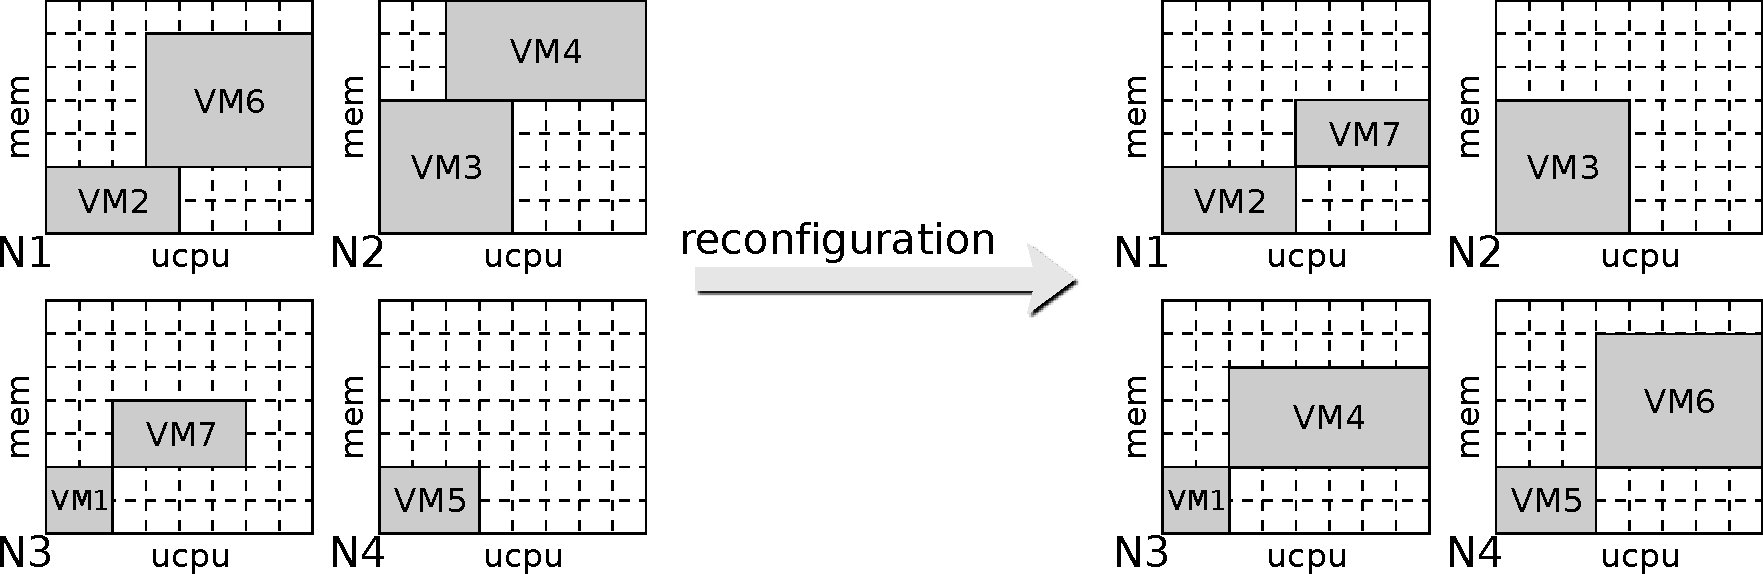
\includegraphics[width=\textwidth]{img/preserve}
\caption{A reconfiguration motivated by \cstr{preserve} constraints.}\label{fig: preserve}
\end{figure}


\begin{reconfPlan}
\centering
\begin{tabular}{ll}
\O & $\rightarrow$ relocate(VM6)\\
!relocate(VM6)\ & $\rightarrow$ relocate(VM7)\\
!relocate(VM7)\ & $\rightarrow$ relocate(VM4)
\end{tabular}
\caption{Event-based reconfiguration plan.}\label{fig: preserve plan}
\end{reconfPlan}


\begin{itemize}
\item \cstr{preserve(\{VM2, VM3\},4,"ucpu")}. This constraint was not satisfied in the source configuration as the
hosting servers of the given VMs do not provide enough resource to them: \cstr{N1} provides 8 unit of
CPU resources but \cstr{VM6} requires 5 units and \cstr{VM2} requires 4 units . In addition, VMs on \cstr{N2} required 10 units of CPU resources. These violation were fixed by relocating \cstr{VM4} and \cstr{VM6} to \cstr{N3} and \cstr{N4}, respectively.
%
However, \cstr{N4} does not initially provides enough resources to host simultaneously \cstr{VM4} and \cstr{VM7}. It has then be decided to relocate first \cstr{VM6} to \cstr{N4}�to liberate enough resource on \cstr{N1} to host \cstr{VM7}. Once this relocation terminated, enough resources were available on \cstr{N3} to
host \cstr{VM4}.

\item \cstr{preserve(\{VM1, VM7, VM5\},2,"mem")}. This constraint was satisfied in the source configuration as
their hosting servers provided enough memory resources to meet their requirement. The constraint is still
satisfied in the destination configuration despite the relocation of \cstr{VM7}.
\end{itemize}

\fullVersion{
\subsection{Model}
\label{preserve: model}
For each d-slice placement variable of the involved VMs,
its resource demand is modified to ask with at least the required amount of resources
if the demand was lesser than the amount to provide.
The constraint is modeled as follow:

\begin{equation*}
\begin{split}
\forall V \in \mathcal{V},\ preserve(V, n) & \triangleq\\
	& \forall v_i \in V, d_i^{cpu} = min(d_i^{cpu}, n)
\end{split}
\end{equation*}

\subsection{Violation Detection}

The detection of misplaced VMs can be made by observing the free resource on the current configuration. For each server, if the VM resource demand is greater than the server capacity then,
VMs will have to move. It is however not possible to check for the VMs that will be relocated in practice 
as this will be a technical choice depending on the global environment. A safe approach is then to consider that every VM on the server may have to be relocated.

\subsection{Availability}

\subsubsection{In {\btrp}}

The \cstr{preserve} constraint is available in {\btrp} since version 2.1. As the resource usage
of the d-slices placement variables is a constant, no specific Choco constraints are required.
Its model is then similar to the one detailed in~\ref{preserve: model}.
}
\subsection{See also}

\subsubsection{Related Constraints}
\begin{itemize}
\item \cstrref{oversubscription}: A constraint made available to the
datacenter administrator to control the resource overbooking on the servers. 
\end{itemize}

\printListOfInheritance{preserve}